\documentclass{article}
\usepackage[utf8]{inputenc}
\usepackage{amsmath}
\usepackage{graphicx}
\usepackage{multicol}
\usepackage{ragged2e}
\usepackage{subcaption}
\usepackage[utf8]{inputenc}
\usepackage[export]{adjustbox}
\usepackage{wrapfig}

\title{
On a mathematical model of the speed for "n" motors on an omnidirectional robot}
\author{Pablo César Ruíz Hernández}
\date{November 2018}
\begin{document}
\begin{multicols}{2}

\maketitle
\section{An Omnidirectional Robot}
In recent years there has been an increase in the presence of omnidirectional drive systems in robotics. These complex systems help robots navigate in a vector space where they can reach any point within a discrete given range.
This paper aims to generalize a mathematical model to describe the behavior of any omnidirectional robot with standard omnidirectional wheels.


\bigskip
\textbf{Omnidirectional Wheels}
\begin{justify}
\textit{Before the mathematical analysis of the drive system it is important to define what an omnidirectional wheel is.}
\bigskip
\end{justify}

An omnidirectional wheel is characterized by the smaller wheels contained within its circumference, each of these smaller wheels move in a perpendicular direction relative to the whole wheel; that is why the omnidirectional drive can be achieved. An example of an omnidirectional wheel can be seen in figure 1.

\bigskip
\bigskip
\bigskip
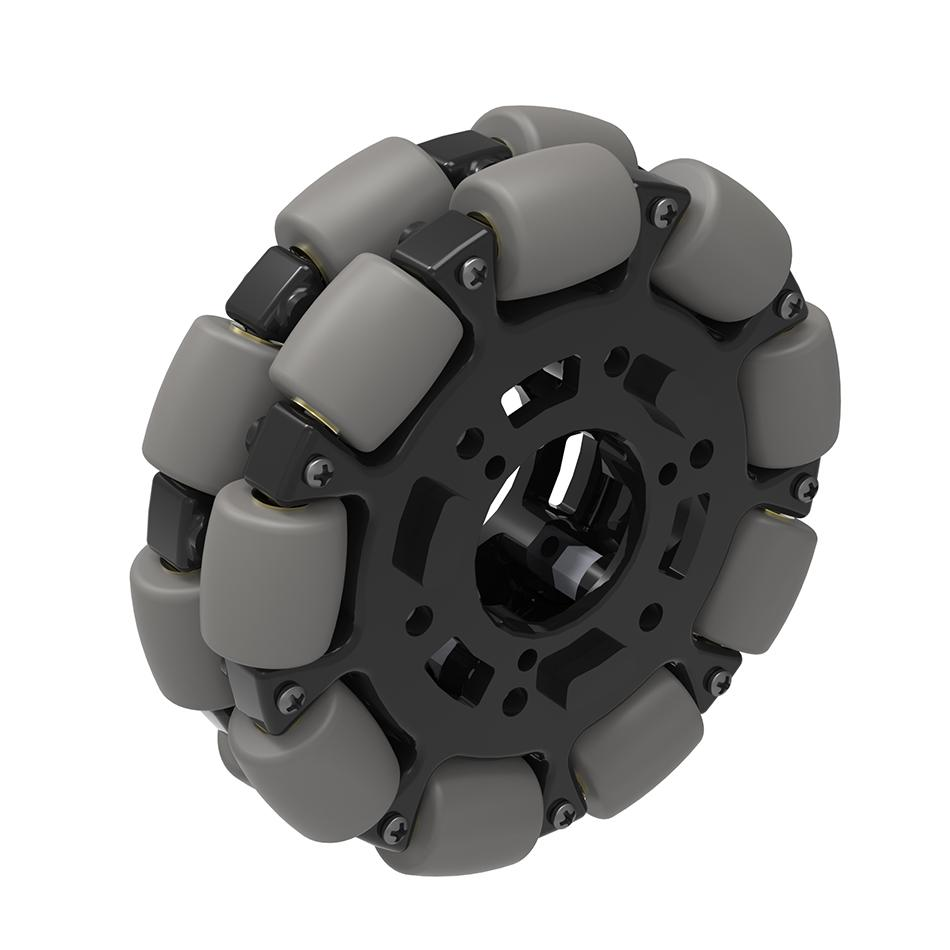
\includegraphics[width=0.5\textwidth, center]{llanta}
\put(-100,0){Figure 1.}

\textbf{Robot Drive}

The most basic robot that can be driven with an omnidirectional drive is a four motor robot with a separation angle $\beta = 45º$ between each motor. Commercial and competitive robots with this kind of setups are very popular. But it's important to acknowledge that the system is not limited to only three or four motors. The amount of motors that an omnidirectional robot can have is restricted by it's size rather than by a convention. That said, we can visualize the robot as in figure 2 and 2.1.

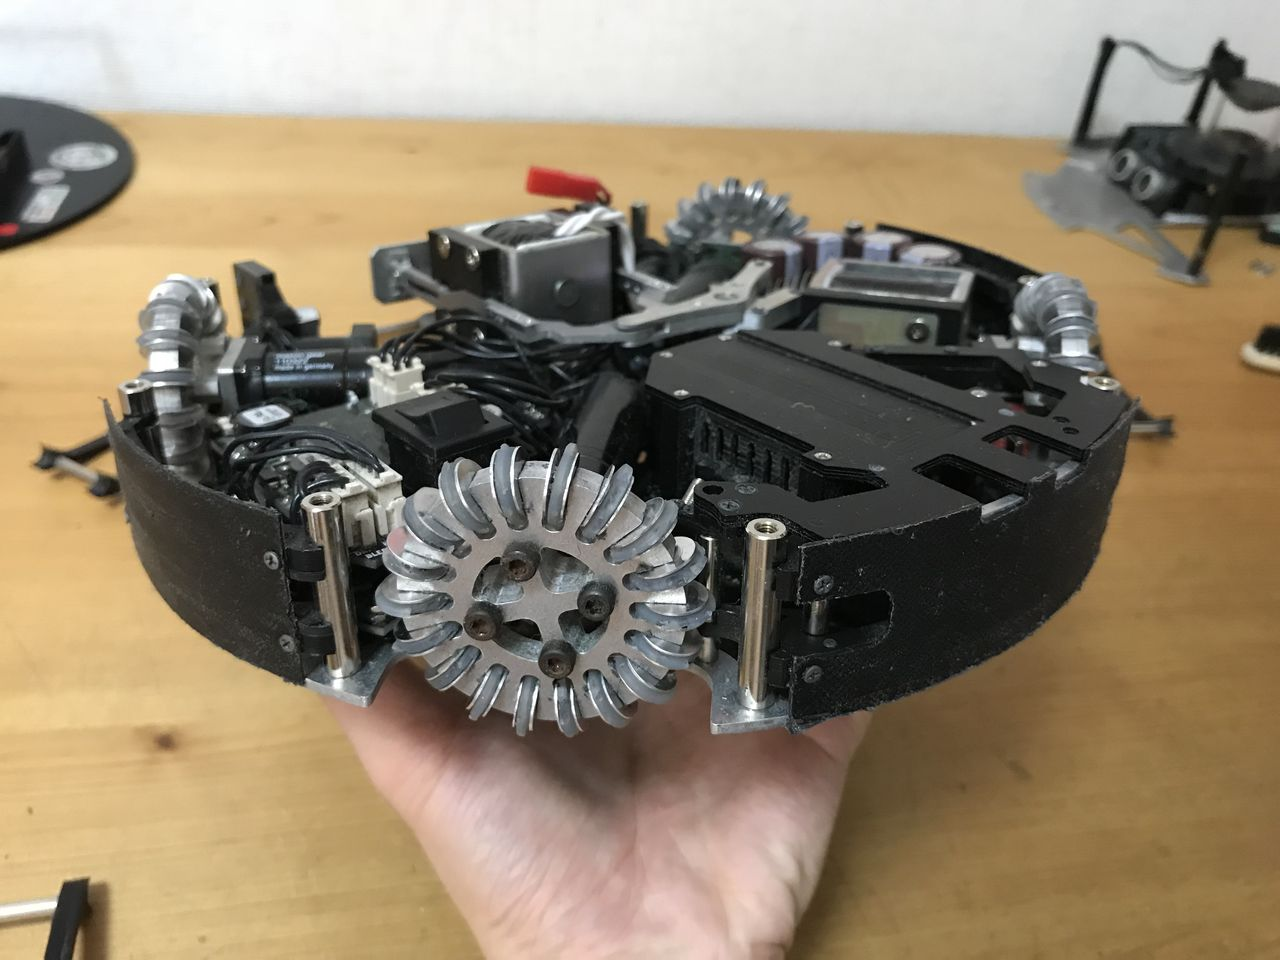
\includegraphics[width=0.4\textwidth, center]{omniRobot}
\put(-100,-10){Figure 2.}
\bigskip

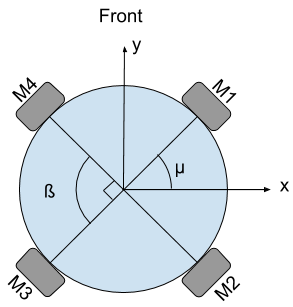
\includegraphics[width=0.4\textwidth, center]{OmniRobotCW}
\put(-120,0){Figure 2.1.}
\bigskip

This particular arrangement offers liberty of displacement to the robot. By having omnidirectional wheels tangent to the circumference of the robot, they can add their forces to get a resultant directional force as described in (1).
\begin{equation}
\sum_{i=1}^{n} \overrightarrow{F}_{M_{i}} = \overrightarrow{F}_{res}
\end{equation}
in (1), $m_{i}$ stands for the $i^{th}$ motor, and n stands for the number of motors in the robot.

\section{Wheel Forces Analysis}
\textbf{Drift force and Motor force}
\bigskip

 It is important to acknowledge that if the wheels used in the robot were not omnidirectional, the robot would experience great friction forces that would lead to damage the system by burning the motors or breaking the wheels.
\bigskip
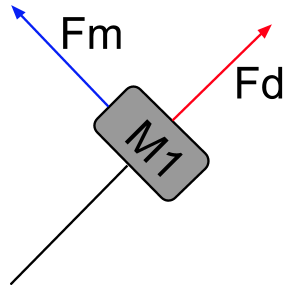
\includegraphics[width=0.4\textwidth, center]{WheelF}
\put(-100,0){Figure 3.}
\bigskip

As seen in figure 3, since omnidirectional wheels have smaller wheels pointing in a perpendicular direction to the motion of the motor, they push all the friction forces obtained by adding the motor friction forces to a drift force. That means that any force (or sum of forces) that is applied to a specific motor in a direction between the motor force and the perpendicular vector to the motor force, will be added directly to the drift force (which is the same as the perpendicular vector to the motor force).
\bigskip

\begin{center}
Let S = $\{M_{i} \mid M_{i} \text{ is the }  i^{th} \text{ motor} \}$
\end{center}

\begin{equation}
\sum_{ x_i \in S \wedge i\neq a} x_i = \overrightarrow{F}_{d_{M_{a}}}
\end{equation}

\bigskip
As described in (2), all the friction forces generated by all the motors except one, push a drift force to that remaining motor. That applies for any motor contained in the robot. 

\section{Motor Forces, Vector Analysis}

We now know that all the motors have two forces, the motor force and the drift force. But since the system remains harmonic in all circumstances so it can move (meaning that every motor depends on each other to drive the robot properly), the functions that describe each motor's movement must be harmonic too. 

Please address figure 4 for a further detailed example. In figure 4 it is clear that motor forces and drift forces add up to direct the robot towards the force's color direction.\\

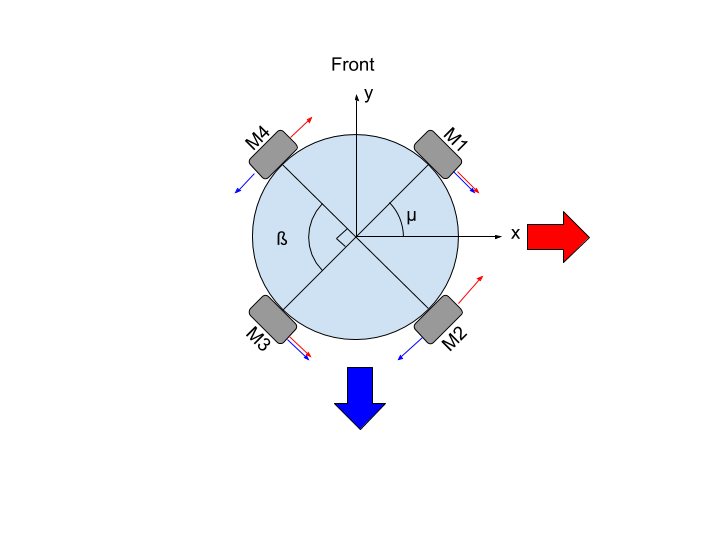
\includegraphics[width=0.5\textwidth, center]{OmniForces.png}
\put(-200,0){Figure 4.}
\bigskip

As seen in figure 4, if it is intended to move the robot towards the right (red arrow), $M_{1}$ and $M_{2}$ must add up towards the same direction whilst $M_{3}$ and $M_{4}$ towards inverse directions. Something similar happens with the blue force. If the direction of the robot is given as a point (x, y) in space, there must be a way to relate the speed of the motors with the direction of that point relative to the center of the robot. That function must be the same as the one that relates the sum of the motor forces as the resultant vector of those forces; where the resultant vector is exactly the same as the direction vector (the vector that extends from the center of the robot to the (x, y) coordinate).\\

\bigskip
The function that describes the speed for each motor given an (x, y) point in the plane is shown in (4), where (x, y) allow us to find $\alpha$ which is the angle between the direction of the motor forces and the desired force (the vector extending from the center of the robot to the (x, y) point).\\

It's trivial to see that 
\begin{equation}
\alpha = \tan{\frac{x}{y}}
\end{equation}

With (3), the general function of the speed of each motor can be expressed as:
\begin{equation}
F_{M_{i}}={-1}^{i+1}velocity\sin(\alpha+\frac{i\pi}{2})
\end{equation}
Where the velocity is an input obtained by the robot controller.\\ 

Which is the same as:
\begin{equation}
F_{M_{i}} = velocity \cdot \frac{d^{i+1}\sin(\alpha + \frac{\pi}{2})}{d\alpha^{i+1}}
\end{equation}

In (4) and (5) every sine function has a $\frac{\pi}{2}$ shift due to the direction of the perpendicular drift force and $\beta$ from figure 2.1 which is the separation angle between each motor axis. The simplification of the addition of the components of the complete force set S in (2), is a $90º$ shift in every motor. 

Which is also the same as:
\begin{equation}
velocity \cdot \frac{d^{i+1}\cos(\alpha)}{d\alpha^{i+1}}
\end{equation}

This homogeneous harmonic relation appears to be quite simple regarding the complexity of such a drive system. At first sight it appears to only sustain with systems with four wheels. But it happens that the function of the direction isn't particular for each motor, but for each quadrant of the circle that is represented by the robot's circumference.
\bigskip

Modifying (2), the general formula for the speed of the $i^{th}$ motor is: 

\begin{center}
Let S = $\{Q_{i+1} \mid Q_{i+1} \text{ is the }  i^{th} \text{ quadrant} \}$
\end{center}

\begin{equation}
\sum_{ x_i \in S \wedge i\neq a} x_i = \overrightarrow{F}_{d_{M_{a}}}
\end{equation}
Where $M_{a}$ is contained in the quadrant $x_{i}$.\\
\begin{justify}
Hence, the most general model of this speed function for each motor would be: 
\end{justify}


\bigskip
\begin{equation}
Speed_{a} = velocity \cdot \frac{d^{i+1}\cos(\alpha+ \beta)}{d\alpha^{i+1}}
\end{equation}
\bigskip

where "i" is the quadrant of the motor, "a" is the number of the motor and $\beta$ is the separation angle between the actual motor and the adjacent motor in a counterclockwise direction.

\bigskip
\bigskip
\end{multicols}
\end{document}